\chapter{Sequential Digital Systems}
\section{Digital Memory}
% second part of video 22
All the previous circuits were "combinational" circuits. This means that identical inputs will always produce identical outputs. These circuits are useful for straightforward applications such as a door bell, turning on a light, an alarm, \ldots i.e. simple circuits that don't need a memory. Another application is the implementation of mathematical function as in a calculator. They can however not be used for more complicated functions like event counting, or for state machines like processors: devices that have a state, i.e. some internal circuitry determines in which state they are.\\
\emph{Sequential Logic} adds a new dimension to the use of digital circuits: they contain a memory. You can now work with circuits whose response is "event dependent", like electronic locks, counters or state machines: the way they behave not only depends on the current input, but also on the past and the inputs they received previously.

\begin{figure}[h!]
	\centering
	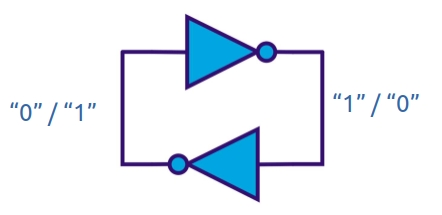
\includegraphics[width=9cm]{figures/ch17/mem_element.jpg}
	\caption{}
	\label{fig:mem_element}
\end{figure}

A simple memory element, capable of storing one bit of information, is shown in figure \ref{fig:mem_element}. It are essentially two NOT-gates back-to-back. If the input of one gate is "0" (LOW) the output will be "1" (HIGH). This signal is then propagated through the other NOT-gate to the input of the first one. In this way, the signal is sustained and the element remains in memory. This is also called a \emph{flip-flop} or \emph{latch}: a circuit that has two stable states that can store state information.\\
The problem however is that there is no mechanism to change the memory. This can be solved with an SR-flip-flop.

\section{SR Flip-Flop}
An SR flip-flop replaces the two NOT-gates from figure \ref{fig:mem_element} with two NAND-gates as in figure \ref{fig:SR_FF}. If input $S$ ("Set") and $R$ ("Reset") are both low, nodes $X$ and $Y$ are high. When one input of a NAND-gate is high, the gate acts as a NOT-gate on the other input: $\overline{1 \cdot A} =\overline{A}$. So to two NAND-gates with each an input at 1 acts as the connected NOT-gates in figure \ref{fig:mem_element}. This means that the bit present in memory $Q$ is sustained. The other output is always not-$Q$: $\overline{Q}$.
\begin{figure}[h!]
	\centering
	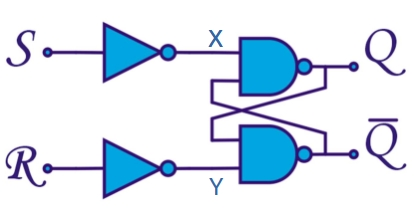
\includegraphics[width=8cm]{figures/ch17/SR_FF.jpg}
	\caption{}
	\label{fig:SR_FF}
\end{figure}
When $S$ is high and $R$ is low, node $X$ is low and $Q$ becomes high, irrespective of what the memory state was. Consequently, the other NAND-gate has two high inputs and produces $\overline{Q} = 0$. When $R$ is high and $S$ is low, $\overline{Q}$ becomes high and $Q = 0$.\\
It is not allowed to make both inputs high: in that case, both $Q$ and $\overline{Q}$ become high. After $S$ and $R$ return to low, there is a conflict: only one of them can stay high in the end. This will be the one for which the signal propagates the fastest through the different gates. This is hard to predict, so we don't know what will be the memory state of the latch - an unacceptable situation.\\
The truth table is shown in figure \ref{fig:SR_FF2}. Note how the first line means that memory state $Q$ is unchanged. "NA" stands for "Not Allowed".\\
The symbols for clocked and unclocked SR flip-flop are represented in figure \ref{fig:SR_FF3}. The difference is that a clocked flip-flop has an additional input for a clock signal: a block signal that alternates between low and high with a constant period, for instance generated by a relaxation oscillator from chapter \ref{sec:relaxation}. A transition of the memory state will only happen at a rising edge of the clock signal, i.e. only the values that $S$ and $R$ have at the time of the rising edge matter. In an unclocked flip-flop, the output changes whenever $S$ or $R$ are set to high. The use of a clock synchronizes the behavior of the flip-flop, and avoids problems when they are used in larger circuits. It is therefore recommended to always use the clocked version.\\
\begin{minipage}{.5\textwidth}
	\centering
	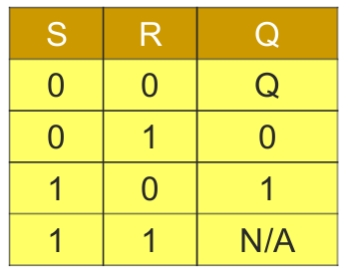
\includegraphics[width=4cm]{figures/ch17/SR_FF2.jpg}
	\captionof{figure}{}
	\label{fig:SR_FF2}
\end{minipage}%
\begin{minipage}{.5\textwidth}
	\centering
	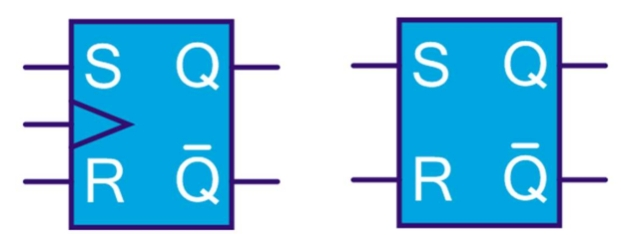
\includegraphics[width=6cm]{figures/ch17/SR_FF3.jpg}
	\captionof{figure}{}
	\label{fig:SR_FF3}
\end{minipage}
For the clocked version, we can also determine the \emph{transition table}. It shows how the input has to be set to obtain a specific output $Q_{next}$ after the next transition, given the current (or present) output $Q_{present}$. For the SR flip-flop, the transition table is given in figure \ref{fig:SR_FF4}. An "X" entry means that the value can be either 0 or 1 - it's basically a "don't care". Convince yourself that this table gives the same results as the one in figure \ref{fig:SR_FF2}.

\begin{figure}[h!]
	\centering
	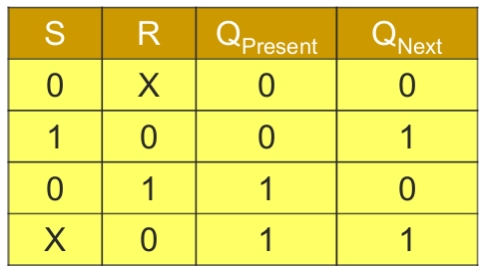
\includegraphics[width=5cm]{figures/ch17/SR_FF4.jpg}
	\caption{}
	\label{fig:SR_FF4}
\end{figure}

\section{D-Latch}
\label{sec:dlatch}

A D-latch is an adaptation of the SR flip-flop, as in figure \ref{fig:D_FF1}. It works as follows:
\begin{itemize}
	\item When input $W$ is low, both nodes $X$ and $Y$ are high, so the NAND-gates act as interconnected NOT-gates and the existing memory bit $Q$ is maintained.
	\item When $W$ is high, node $X$ is equal to $\overline{D}$ and $Y = \overline{X} = D$. So if $D = 1 \rightarrow X = 1 \rightarrow Q = 1$ and if $D = 0 \rightarrow Y =  0 \rightarrow \overline{Q} = 1$ and $Q = 0$, i.e. when $W = 1$, $Q$ takes the value of the data bit $D$ (so "D" stands for "Data").
\end{itemize}
 Note how this topology avoids that $X = Y = 0$, the situation of the SR flip-flop that is not allowed. The symbol is shown in figure \ref{fig:D_FF2}.

\begin{minipage}{.5\textwidth}
	\centering
	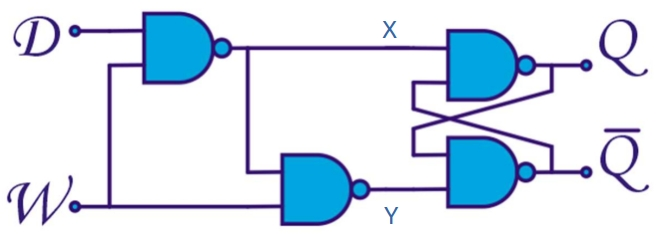
\includegraphics[width=8cm]{figures/ch17/D_FF1.jpg}
	\captionof{figure}{}
	\label{fig:D_FF1}
\end{minipage}%
\begin{minipage}{.5\textwidth}
	\centering
	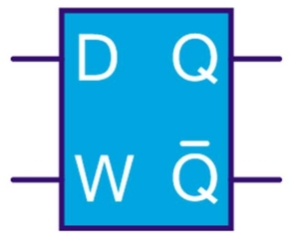
\includegraphics[width=3cm]{figures/ch17/D_FF2.jpg}
	\captionof{figure}{}
	\label{fig:D_FF2}
\end{minipage}

A very useful change to the D flip-flop is the clocked configuration, where input $W$ is replaced by a clock entrance. Input $D$ will only be transferred to the memory state $Q$ on the rising edge of the clock signal - it is edge-triggered.

\begin{minipage}{.5\textwidth}
	\centering
	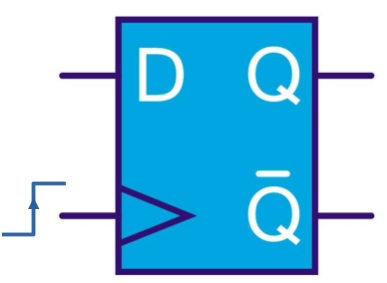
\includegraphics[width=3cm]{figures/ch17/D_FF3.jpg}
	\captionof{figure}{}
	\label{fig:D_FF3}
\end{minipage}%
\begin{minipage}{.5\textwidth}
	\centering
	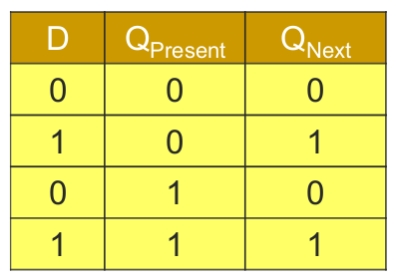
\includegraphics[width=4cm]{figures/ch17/D_FF4.jpg}
	\captionof{figure}{}
	\label{fig:D_FF4}
\end{minipage}

An edge-triggered D-flipflop is often used as a delay element in a digital filter, as in figure \ref{fig:D_FF5}. The input signal propagates through the delay line and is moved one step to the right at each rising edge of the clock. So the value $x(t)$ at time $t$ at the input of the line is available after one period $T$ at the output of the first D-flipflop, at the output of the second flipflop after $2\;T$, and so on.

\begin{figure}[h!]
	\centering
	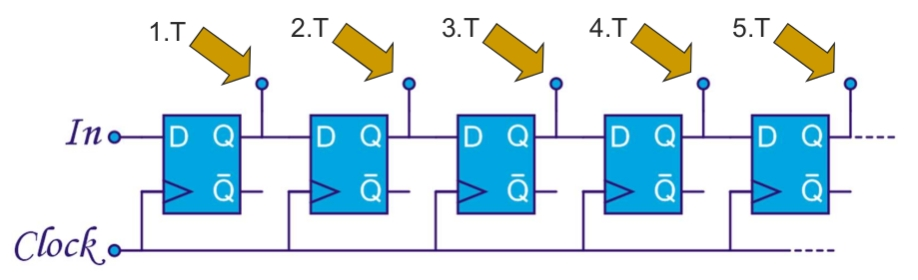
\includegraphics[width=14cm]{figures/ch17/D_FF5.jpg}
	\caption{}
	\label{fig:D_FF5}
\end{figure}

A finite impulse response (FIR) filter is a digital filter that computes an output signal $y[n]$ based on the current and previous values of input $x[n]$:
$$ y[n] = a_0 x[n] + a_1 x[n-1] + a_2  x[n-2] + \ldots + a_{N-1} x[n-N+1]$$
where $N$ is the number of so-called tabs. For instance, if $N = 2$ and $a_0 = a_1 = 1/2$, we have an averaging filter of order $1$, which removes the higher frequency components in the signal. All $x[n-k]$ tabs are supplied by a D-flipflop delay line. Digital filters will be studied in the course on Signals \& Systems (ES311).

\subsection{Implementation of the Edge-trigger}
To implement the D-flipflop with an edge trigger, we use the circuit from \ref{fig:edge_trigger1}. The part at the left is the \emph{master}, the part connected to the output is the \emph{slave}. Both can operate as a memory element, and each does this during part of the clock cycle. \\
\begin{figure}[h!]
	\centering
	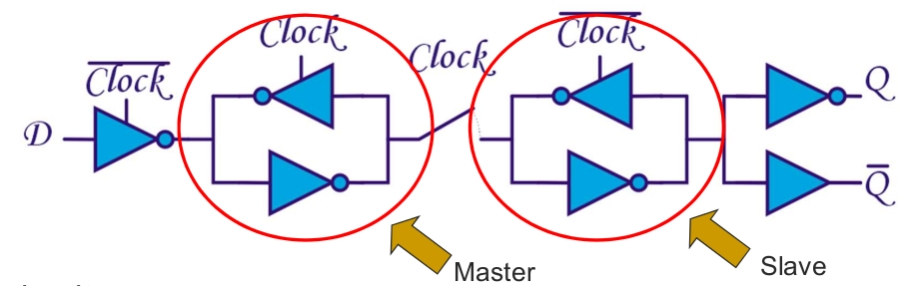
\includegraphics[width=12cm]{figures/ch17/edge_trigger1.jpg}
	\caption{}
	\label{fig:edge_trigger1}
\end{figure}
Their operation is controlled by NOT-gates with inhibitor gates (\ref{sec:inhibition}) so they behave differently during different parts of the clock cycle:
\begin{enumerate}
	\item \underline{When the clock is low}:\\
	The circuit can be reduced to the one in figure \ref{fig:edge_trigger2}. The master is connected to the input and follows the input through two NOT-gates in series. He is disconnected from the slave, which operates as a memory element with two active NOT-gates back-to-back, and retains thus the value it has.
	\begin{figure}[h!]
		\centering
		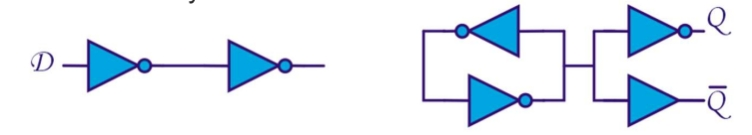
\includegraphics[width=12cm]{figures/ch17/edge_trigger2.jpg}
		\caption{}
		\label{fig:edge_trigger2}		
	\end{figure}

	\item \underline{When the clock is high}:\\
	When the clock signal goes from low to high (i.e. the rising edge) the master is disconnected from the input and connected to the slave. The master is transformed in a memory element and retains the value it saw at the input just before the rising edge. This value is transmitted through the slave, which in turn is now two NOT-gates in series, to outputs $Q$ and $\overline{Q}$, as in figure \ref{fig:edge_trigger3}.
	\begin{figure}[h!]
		\centering
		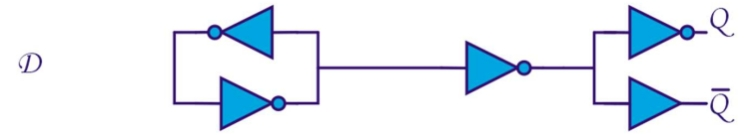
\includegraphics[width=12cm]{figures/ch17/edge_trigger3.jpg}
		\caption{}
		\label{fig:edge_trigger3}		
	\end{figure}
\end{enumerate}
The consequence is that the data $D$ that is present at the input at the rising clock edge, is transferred to the output and stays there for the entire clock cycle.\\
An SR flipflop can also be implemented with and edge trigger with the circuit in figure \ref{fig:edge_trigger4}. When the clock is low, the initial part is an odinary (not edge-triggered) SR flipflop as we saw before. The slave is then just a memory element. When the clock goes high, $S$ and $R$ are disconnected from the circuit, and the inputs of the NAND-gates are connected to the supply (high) so the gates function as NOT-gates. The master becomes the memory element and its bit is transferred via the slave to the output.

\begin{figure}[h!]
	\centering
	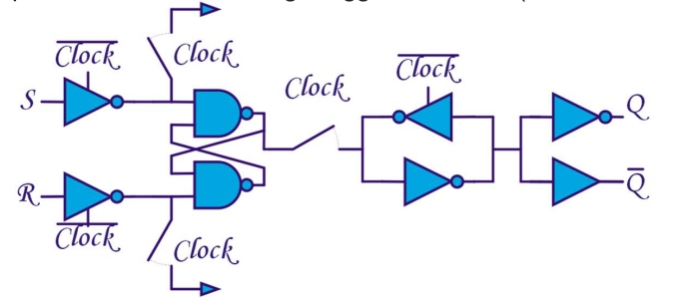
\includegraphics[width=12cm]{figures/ch17/edge_trigger4.jpg}
	\caption{}
	\label{fig:edge_trigger4}		
\end{figure}

\section{JK Flip Flop}

The JK flipflop is an extension of the SR flipflop, where also the undefined input can be used. The consequence is that when the two input $J$ and $K$ are the low (either low or high), the memory state $Q$ is retained, but when they are both equal to one, the memory state is flipped. The truth table is shown in figure \ref{fig:JK_FF2}. The symbol of this fliflop is exactly the same as for the SR flipflop, but with other names for the inputs - see figure \ref{fig:JK_FF2}. As before there is an clocked and unclocked version - obviously the clocked version is preferred.

\begin{minipage}{.5\textwidth}
	\centering
	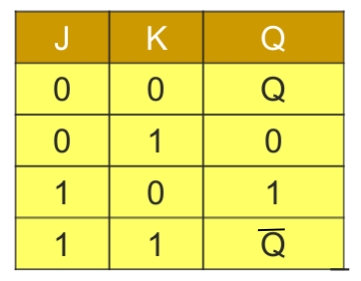
\includegraphics[width=4cm]{figures/ch17/JK_FF2.jpg}
	\captionof{figure}{}
	\label{fig:JK_FF2}
\end{minipage}%
\begin{minipage}{.5\textwidth}
	\centering
	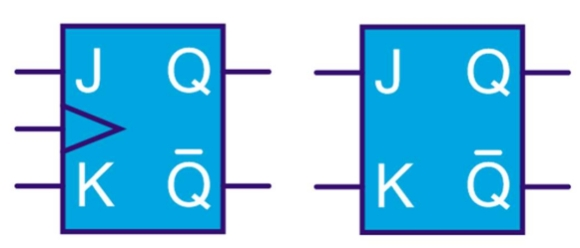
\includegraphics[width=5cm]{figures/ch17/JK_FF1.jpg}
	\captionof{figure}{}
	\label{fig:JK_FF1}
\end{minipage}

The transition table for the clocked version is shown in figure \ref{fig:JK_FF3}. For example, if we have a zero in memory and we want to keep it, as in the first line, we either keep the current memory with $J=0, K=0$, or we set the memory to zero: $J=0, K=1$. So to have this transition, $J$ should be zero but hte value of $K$ doesn't matter ("X" stands for "Don't care"). The reasoning for other lines is similar.\\
A possible implementation can be found in figure \ref{fig:JK_FF4}. For the first three lines of the truth table, there is no problem and we can just either generate the memory state with the master based on the input ("Set": $J=1", "K=0"$ or "Reset": $J=0, K=1$) or keep the value in memory $J = K = 0$. But if $J=K=1$, we need to invert the value in memory, so we have to fetch it and invert it. 

%\textbf{TODO:} explain in more detail.

\begin{figure}[h!]
	\centering
	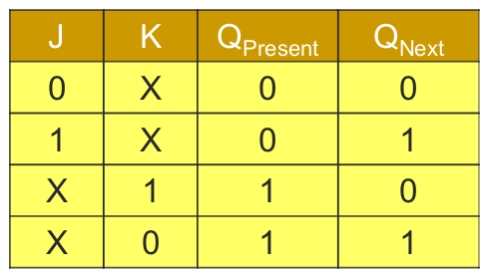
\includegraphics[width=6cm]{figures/ch17/JK_FF3.jpg}
	\caption{}
	\label{fig:JK_FF3}
\end{figure}

\begin{figure}[h!]
	\centering
	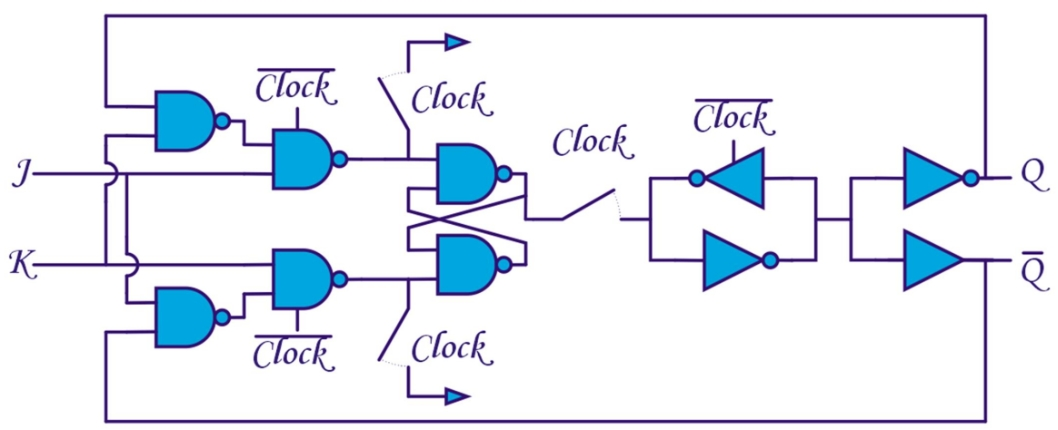
\includegraphics[width=12cm]{figures/ch17/JK_FF4.jpg}
	\caption{}
	\label{fig:JK_FF4}
\end{figure}

\section{Applications}
We present in this section two small applications where memory elements are used: a simple counter and a register. In the next section, we discuss the sequential circuit design method, which is a principled approach to implement (complex) sequential systems.

\subsection{The Counter}

\begin{minipage}{.7\textwidth}
	A simple counter can be implemented with the circuit in figure \ref{fig:counter1}. It is a counter for 4 bits, so it counts from $0$ to $2^4 - 1 = 15$ in binary.\\
	All flip-flops have initially a zero memory state. The $J$ and $K$ inputs for all flip-flops are both set to $1$ which means that the memory value will be flipped at each rising edge at the clock port. The first flip-flop, which contains the least significant bit, flips every time the input signal goes from low to high. The output $\overline{Q}$ of this flip-flop is the clock input of the next one, so the second flip-flop flips when the first bit $Q_0$ goes from $1$ to $0$. This repeats for every two flip-flops and means that every flip-flop flips once for every two flips of the previous one.\\
	The result is that the the output signal that is produced is an increasing sequence of binary numbers, as in figure \ref{fig:counter2}, up until $15$ and then the entire sequence starts again. This counter can easily be extended to higher numbers.
\end{minipage}
\begin{minipage}{.3\textwidth}
	\centering
	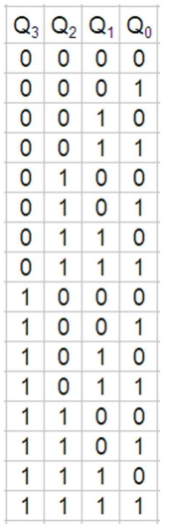
\includegraphics[height=7cm]{figures/ch17/counter2.jpg}
	\captionof{figure}{}
	\label{fig:counter2}
\end{minipage}%

\begin{figure}[h!]
	\centering
	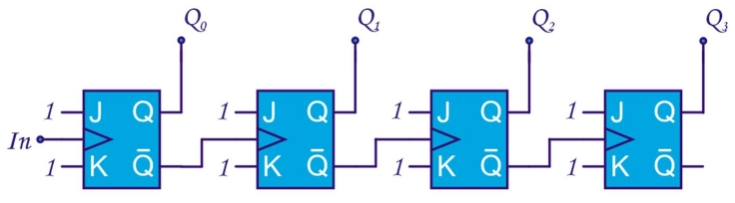
\includegraphics[width=12cm]{figures/ch17/counter1.jpg}
	\caption{}
	\label{fig:counter1}
\end{figure}

\subsection{The Register}
% video 23 20:38

\begin{minipage}{.6\textwidth}
	A register is similar to memory, but has typically more functions, i.e. it can work in several modes. The register we show here has $4$ D-flipflops as memory cells and has $2$ modes: parallel and series (or shift). The mode is set by a multiplexer such as we saw in section \ref{sec:multiplexer}. \\
	In parallel ($P$) mode the multiplexers put the inputs $P_0$ to $P_3$ directly on the $D$ input pin of the latch. These values are thus read into memory whenever the $W$ input is high.\\
	In series ($S$) mode, the initial value $S$ is read into the first flip-flop, and every other flip-flop changes its value to the one of the previous latch - when $W$ is high, off course. \\
	A register is not really used as a memory: it is lot smaller and can also perform small operations. The series (or shift) operation from the register on the right, for instance, corresponds to a (binary) multiplication by $2$ when the initial value $S$ is zero. A register is usually added to an ALU (Arithmetic-Logic Unit) to memorize small amounts of data that are needed for intermediary steps in calculations.
\end{minipage}
\begin{minipage}{.5\textwidth}
	\centering
	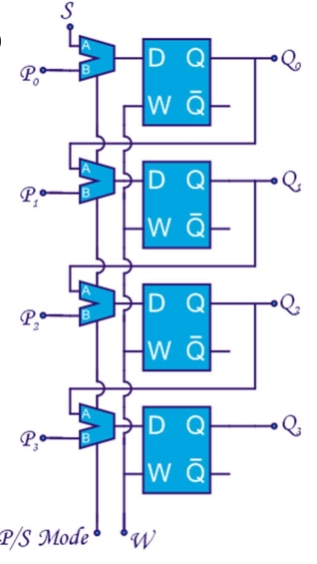
\includegraphics[width=5cm]{figures/ch17/register1.jpg}
	\captionof{figure}{}
	\label{fig:register1}
\end{minipage}%

\section{Sequential Circuit Design}
\label{sec:seq_design}

\begin{minipage}{.6\textwidth}
A sequential circuit consists of three elements:
\begin{enumerate}
	\item A flip-flop array, that contains a number of flip-flop memory cells and retains the state of the circuit.
	\item I/O logic, a combinational circuit that generates the output based on the input and the memory.
	\item the next-state logic, another combinational circuit that transforms the circuit input into the J/K, S/R or D inputs for the flip-flops used in the array such that the circuit will evolve to the next state.
\end{enumerate}
The memory state makes the analysis of a sequential circuit more difficult than a combinational circuit. To perform this analysis, we rely on a \emph{state diagram}.
	
\end{minipage}
\begin{minipage}{.4\textwidth}
	\centering
	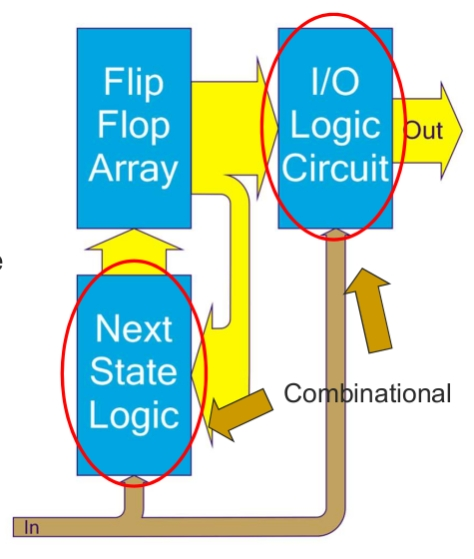
\includegraphics[height=7cm]{figures/ch17/design1.jpg}
	\captionof{figure}{}
	\label{fig:design1}
\end{minipage}%

A state diagram represents the state a circuit is in, the possible inputs (if there are any) and where to system will evolve to, based on the present state and the input - i.e. what will be the next state. We represent the states of the system as circles containing the state name, and the transitions as arrows between states. An arrow is associated with the current input and the output of that transition. Figure \ref{fig:design2} shows the state diagrams for SR, JK and D flip-flops. Obviously, each flip-flop has $2$ states ($Q=0$ and $Q=1$).

\begin{figure}[h!]
	\centering
	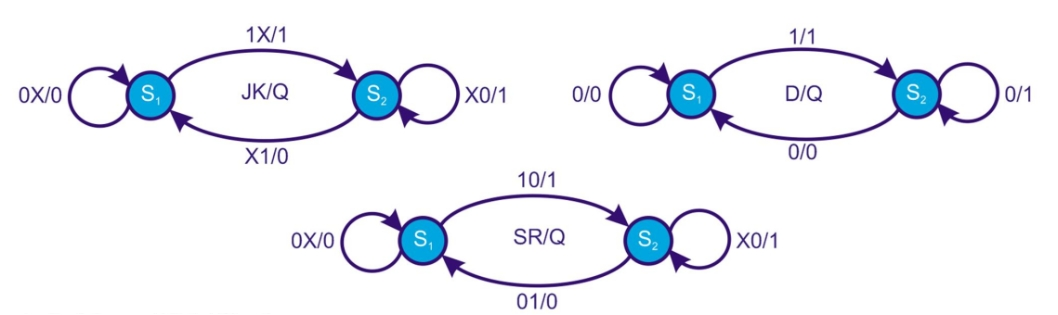
\includegraphics[width=12cm]{figures/ch17/design2.jpg}
	\caption{}
	\label{fig:design2}
\end{figure}

Some other examples are:
\begin{enumerate}
	\item \textbf{Sequence detector} (figure \ref{fig:design3})\\
		\begin{figure}[h!]
			\centering
			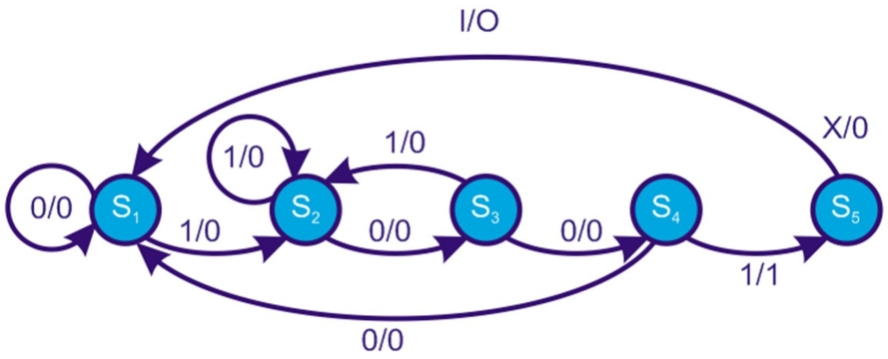
\includegraphics[width=9cm]{figures/ch17/design3.jpg}
			\caption{}
			\label{fig:design3}
		\end{figure}
		This circuit detects a specific sequence in an input bitstream. Specifically, the detected sequence in figure \ref{fig:design3} is "1001". State $S_1$ is the start state, $S_2$ is the state after observing a $1$, $S_3$ the state after "10" and so on. If a bit that is not part of the sequence is observed, two things can happen: if this bit is a 0 the system returns to start state $S_1$, but if it is a 1, it can be the start bit of a new "1001" sequence and the system moves to state $S_2$. After a sequence "1001" is observed, the output goes high (see the transition from $S_4$ to $S_5$) and the system returns to $S_1$.\\
		Because there are $5$ states, we need $3$ flip-flops to represent them.
	\item \textbf{Binary Coded Decimal (BCD) counter} (figure \ref{fig:design4})\\
	This is a counter that goes from $0$ to $9$ and then resets to $0$.  It requires no input and the output is the value of the next state. This choice of output avoids additional logic to transform the state value to the output. An extension is an up-and-down counter, where a input $0$ keeps counting up, and a input $1$ counts down as in figure \ref{fig:design5}. Because there are $10$ states, we need $4$ flipflops.\\
	\begin{minipage}{.5\textwidth}
		\centering
		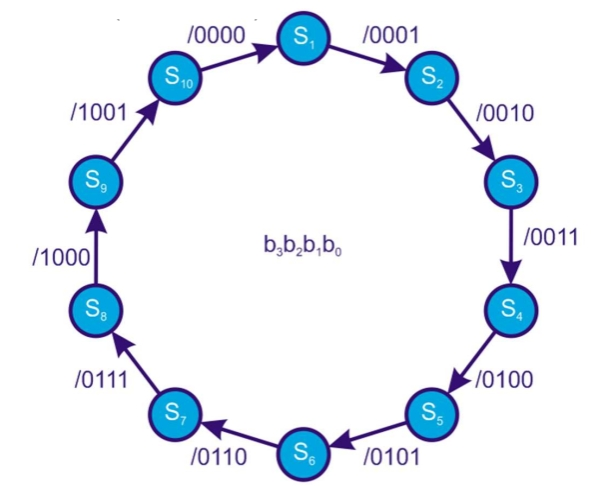
\includegraphics[width=5.5cm]{figures/ch17/design4.jpg}
		\captionof{figure}{}
		\label{fig:design4}
	\end{minipage}%
	\begin{minipage}{.5\textwidth}
		\centering
		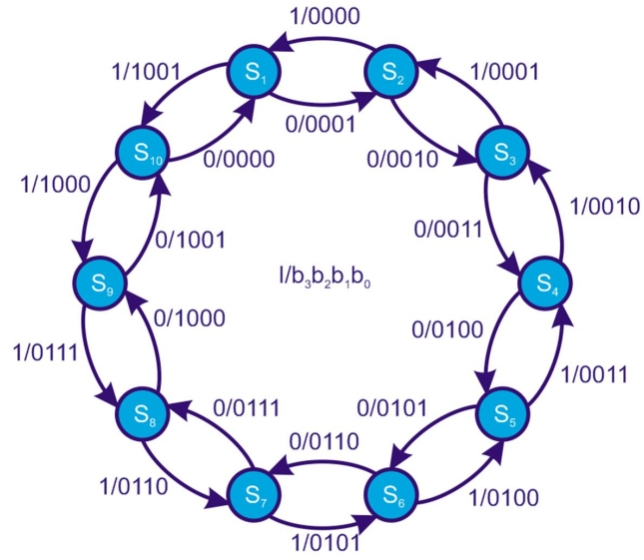
\includegraphics[width=5.5cm]{figures/ch17/design5.jpg}
		\captionof{figure}{}
		\label{fig:design5}
	\end{minipage}
\end{enumerate}

\subsection{Example: An SR-FF using a D-FF}
We will walk through an example to illustrate the sequential design procedure. The goal is to make an SR flip-flop based on a D flip-flop.\\
The design procedure goes as follows:
\begin{enumerate}
	\item Draw the state diagram, as below. 
	\begin{figure}[h!]
		\centering
		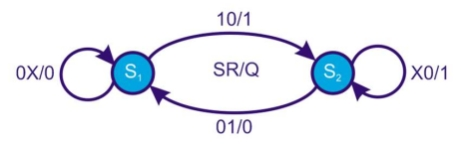
\includegraphics[width=7cm]{figures/ch17/design6.jpg}
		\caption{}
		\label{fig:design6}
	\end{figure}
	\item Derive the transition ("Present-Next state") table. The third column should be interpreted as: if I'm in state $S_1$, where do I move to with inputs $S$ and $R$. Same goes for the last column.
	\begin{figure}[h!]
		\centering
		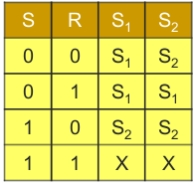
\includegraphics[width=4cm]{figures/ch17/design7.jpg}
		\caption{}
		\label{fig:design7}
	\end{figure}
	From this table, we determine the number of flip-flops we need. The answer is $1$ because there are only $2$ states.
	\item Define for each state the state $F_i$ of the flip-flop and the output $Q$ generated from $F_i$. Whenever possible, we choose $Q = F_i$. The states of the D flipflop are either 0 or 1. We match the outputs $Q$ of the resulting SR FF directly to these states.\\
	\begin{minipage}{.5\textwidth}
		\centering
		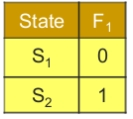
\includegraphics[width=3cm]{figures/ch17/design8.jpg}
		\captionof{figure}{}
		\label{fig:design8}
	\end{minipage}%
	\begin{minipage}{.5\textwidth}
		\centering
		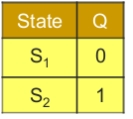
\includegraphics[width=3cm]{figures/ch17/design9.jpg}
		\captionof{figure}{}
		\label{fig:design9}
	\end{minipage}%
\begin{comment}
	\item The next step is a complete state table. This table contains all required information: (1) the possible inputs $S$ and $R$ (2) combined with  the different possible (present) states $F_{1,p}$, (3) the different 'next' states $F_{1,n}$ resulting from these states and inputs and (4) the settings of the input of the D-FF to go from the present to the next state.\\
\end{comment}
	\item The next step is a complete state table. This table contains all required information:
	\begin{enumerate}
		\item the possible inputs $S$ and $R$,
		\item combined with  the different possible (present) states $F_{1,p}$,
		\item the different 'next' states $F_{1,n}$ resulting from these states and inputs,
		\item the settings of the input of the D-FF to go from the present to the next state.
	\end{enumerate}
	\begin{figure}[h!]
		\centering
		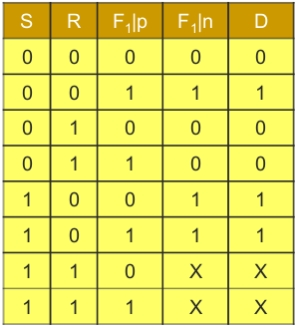
\includegraphics[width=5cm]{figures/ch17/design10.jpg}
		\caption{}
		\label{fig:design10}
	\end{figure}
	\item We construct the Karnaugh table to generate the combinational circuit to produce the input $D$ of the D-flipflop. The inputs are $S$ and $R$ and the present state $F_{1,p}$. The resulting equation is $D = S + \overline{R}\cdot F$.
	\begin{figure}[h!]
		\centering
		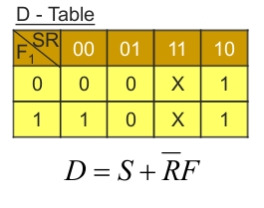
\includegraphics[width=4cm]{figures/ch17/design11.jpg}
		\caption{}
		\label{fig:design11}
	\end{figure}
	\item Based on this expression, we can generate the circuit, with the required flipflops, as in figure \ref{fig:design12}.
	\begin{figure}[h!]
		\centering
		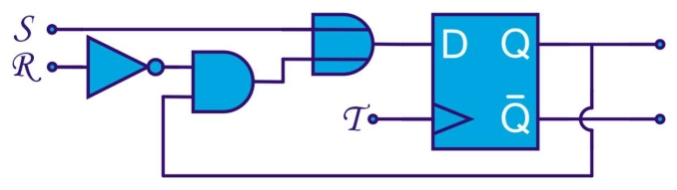
\includegraphics[width=10cm]{figures/ch17/design12.jpg}
		\caption{}
		\label{fig:design12}
	\end{figure}
\end{enumerate}
%More elaborate examples can be found in appendix \ref{app:design_examples}.

\section{Memory Types}
We give a brief overview of memory types found in modern hardware devices.
\subsection{Static RAM}
Static RAM (SRAM) is a type of computer memory that uses a flip-flop circuit to store each bit of data. SRAM is called "static" because it doesn't need to be periodically refreshed like dynamic RAM (DRAM). This means that SRAM is generally faster and more reliable than DRAM.\\
SRAM is commonly used as a cache memory in computer systems. It is also used in certain specialized applications where high speed and low power consumption are critical, such as in aerospace and military systems.\\
One of the key advantages of SRAM is its speed. SRAM can access data in just a few nanoseconds, which makes it ideal for applications that require high performance. However, SRAM is also more expensive than DRAM and requires more power, which limits its use in some applications.\\
Another advantage of SRAM is its durability. Since each bit of data is stored using a flip-flop circuit, it remains in place as long as power is applied to the memory chip. This makes SRAM ideal for applications that require data to be stored for long periods of time, such as in embedded systems or digital signal processing.\\
Overall, SRAM is a powerful and flexible type of computer memory that is used in a wide range of applications where high speed, low power consumption, and durability are important factors.

\subsection{Dynamic RAM}
Dynamic RAM (DRAM) is a type of computer memory that stores each bit of data as a charge on a capacitor within an integrated circuit. DRAM is called "dynamic" because the charge on each capacitor gradually leaks away over time, and needs to be periodically refreshed to prevent data loss. This means that DRAM is generally slower and less reliable than SRAM.\\
DRAM is the most common type of memory used in modern computers. It is used for main memory, which is the memory that the computer uses to store the programs and data that are currently being used.\\
One of the key advantages of DRAM is its cost. DRAM is cheaper than SRAM and requires less power, which makes it ideal for applications that require large amounts of memory, such as personal computers.\\
However, DRAM is also slower than SRAM, with access times typically in the range of tens of nanoseconds. This means that it is less suitable for applications that require high performance, such as in embedded systems or digital signal processing.\\
Another disadvantage of DRAM is its volatility. Since each bit of data is stored as a charge on a capacitor, the data is lost when power is removed from the memory chip. This means that DRAM is not suitable for applications that require data to be stored for long periods of time without power, such as in embedded systems or digital signal processing.\\
Overall, DRAM is a cost-effective and widely used type of computer memory that is ideal for applications that require large amounts of memory at an affordable price.\\

\subsection{Read-Only Memory}
Read-only memory (ROM) is a type of computer memory that is pre-programmed with data that cannot be modified or changed. This type of memory is commonly used for storing firmware and other low-level system information that is critical for the proper functioning of a computer or other electronic device.\\
There are several different types of ROM, including PROM, EPROM, and EEPROM. Here are the key differences between these three types:

\begin{itemize}
	\item PROM (Programmable Read-Only Memory): This type of ROM is programmed once by the manufacturer, using a special device called a PROM programmer. Once programmed, the data in a PROM chip cannot be changed or erased. PROMs are commonly used for storing firmware and other fixed data that is unlikely to change.

	\item EPROM (Erasable Programmable Read-Only Memory): This type of ROM can be erased and reprogrammed using ultraviolet light. EPROM chips have a small window on top that allows the ultraviolet light to reach the memory cells. To erase an EPROM chip, it must be exposed to UV light for several minutes. Once erased, new data can be programmed into the chip using a PROM programmer. EPROMs are commonly used for development purposes and in systems where the firmware may need to be updated.

	\item EEPROM (Electrically Erasable Programmable Read-Only Memory): This type of ROM can be erased and reprogrammed electronically, without the need for UV light. EEPROMs are commonly used for storing small amounts of data that may need to be updated periodically, such as configuration settings or user preferences. EEPROMs are slower than other types of ROM and have a limited number of write cycles, meaning that they can only be reprogrammed a certain number of times before they wear out.

\end{itemize}
